
%
% Optional reading
%

\begin{frame}[plain,c]
\begin{center}
{\Huge \bf Optional reading for Lecture \thislecture}
\end{center}
\end{frame}


%
%
%

\begin{frame}{Electric dipole field}

\begin{columns}
  \begin{column}{0.20\textwidth}
   \begin{center}
     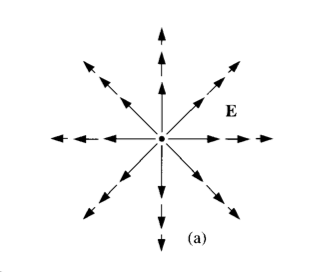
\includegraphics[width=0.99\textwidth]{./images/schematics/electric_field_pos_point_charge.png}\\
   \end{center}
  \end{column}
  \begin{column}{0.80\textwidth}
     As we know, the potential field $V(\vec{r})$ due to an
     {\bf electric monopole} (i.e. a point charge q) has an $1/r$ dependence:
     \begin{equation*}
         V = \frac{1}{4\pi\epsilon_0} \frac{q}{r}
     \end{equation*}
     Consequently, its electric field $\vec{E}(\vec{r})$ ($\vec{E} = -\vec{\nabla}V$)
     has an $1/r^2$ dependence.
  \end{column}
\end{columns}

\vspace{0.3cm}

\begin{columns}
  \begin{column}{0.80\textwidth}
     We will see that the potential field $V(\vec{r})$ due to an {\bf electric dipole} is
     \begin{equation*}
        {\bf V \approx \frac{1}{4\pi\epsilon_0} \frac{\vec{p} \hat{r}}{r^2} }
     \end{equation*}
     Therefore, it falls off as $1/r^2$, faster than the monopole potential.
     Consequently, the dipole electric field $\vec{E}(\vec{r})$
     has an $1/r^3$ dependence.
  \end{column}
  \begin{column}{0.20\textwidth}
   \begin{center}
     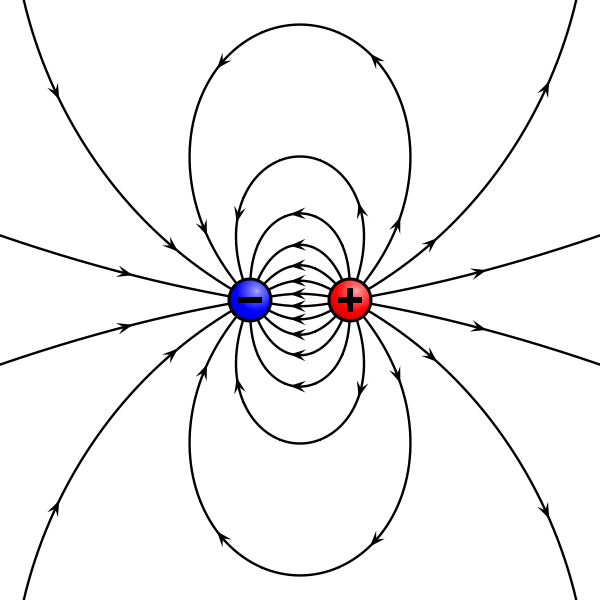
\includegraphics[width=0.90\textwidth]{./images/schematics/electric_dipole_field_lines_2.png}\\
   \end{center}
  \end{column}
\end{columns}

\end{frame}


%
%
%

\begin{frame}{Calculating the electric dipole field}

As we know, the potential field due to a single charge q is given by:
\begin{equation*}
  V = \frac{1}{4\pi\epsilon_0} \frac{q}{r}
\end{equation*}

\vspace{0.1cm}

\begin{columns}
  \begin{column}{0.25\textwidth}
   \begin{center}
     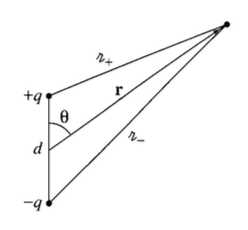
\includegraphics[width=0.95\textwidth]{./images/schematics/electric_dipole_0.png}\\
   \end{center}
  \end{column}
  \begin{column}{0.75\textwidth}
    Now, I have 2 charges: a positive and a negative one. The superposition principle applies.
    The potential at a distance r from the centre of the dipole is:
    \begin{equation*}
      V = \frac{1}{4\pi\epsilon_0} \Big( \frac{q}{r_{+}} - \frac{q}{r_{-}} \Big)
    \end{equation*}
  \end{column}
\end{columns}

\vspace{0.1cm}

I need to express $r_{+}$ and $r_{-}$ in terms of r.
From the law of cosines (generalisation of the Pythagorean theorem):
\begin{equation*}
  r_{+}^{2} = r^{2} + (d/2)^{2} - r \cdot d \cdot cos\theta
            = r^{2} \Big( 1 - \frac{d}{r} cos\theta + \frac{d^2}{4r^2} \Big) \xRightarrow{r>>d}
\end{equation*}
\begin{equation*}
   r_{+}^{2} \approx r^{2} \Big( 1 - \frac{d}{r} cos\theta \Big)
\end{equation*}

\end{frame}

%
%
%

\begin{frame}{Calculating the electric dipole field}

For $r_{-}$, the expressions are similar but involves $cos(\pi - \theta) = -cos\theta$ and,
therefore, there is an extra minus sign.
\begin{equation*}
   r_{-}^{2} \approx r^{2} \Big( 1 + \frac{d}{r} cos\theta \Big)
\end{equation*}

For convenience let me rename the small term involving d/r as $\epsilon$:
\begin{equation*}
  \frac{d}{r} cos\theta = \epsilon
\end{equation*}

We have that
\begin{equation*}
   r_{+}^{2} \approx r^{2} (1 - \epsilon) \Rightarrow
   r_{+} \approx r (1 - \epsilon)^{1/2} \Rightarrow
   \frac{1}{r_{+}} \approx \frac{1}{r} (1 - \epsilon)^{-1/2} \Rightarrow
   \frac{1}{r_{+}} \approx \frac{1}{r} (1 + \frac{1}{2}\epsilon)
\end{equation*}

and, similarly
\begin{equation*}
   \frac{1}{r_{-}} \approx \frac{1}{r} (1 - \frac{1}{2}\epsilon)
\end{equation*}

\end{frame}

%
%
%

\begin{frame}{Calculating the electric dipole field}

Therefore
\begin{equation*}
  \frac{1}{r_{+}} - \frac{1}{r_{-}} \approx
    \Big( \frac{1}{r} (1 + \frac{1}{2}\epsilon) \Big) -
    \Big( \frac{1}{r} (1 - \frac{1}{2}\epsilon) \Big) =
    \frac{1}{r} \epsilon \xRightarrow{\epsilon = \frac{d}{r} cos\theta}
\end{equation*}
\begin{equation*}
  \frac{1}{r_{+}} - \frac{1}{r_{-}} \approx \frac{d}{r^2} cos\theta
\end{equation*}

The electric dipole potential is given by
\begin{equation*}
  V = \frac{1}{4\pi\epsilon_0} \Big( \frac{q}{r_{+}} - \frac{q}{r_{-}} \Big) \Rightarrow
  V \approx \frac{1}{4\pi\epsilon_0} \frac{q d cos\theta}{r^2} \Rightarrow
\end{equation*}
\begin{equation*}
  V \approx \frac{1}{4\pi\epsilon_0} \frac{\vec{p} \cdot \hat{r}}{r^2}
\end{equation*}

So the potential of a dipole falls off as $1/r^2$ ($1/r$ for a monopole).\\
Consequently, the electric field of a dipole falls off as $1/r^3$.\\

\end{frame}

%
%
%

\begin{frame}{The {\em multipole} expansion}

\begin{columns}
  \begin{column}{0.30\textwidth}
   \begin{center}
     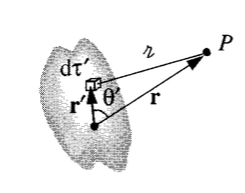
\includegraphics[width=0.99\textwidth]{./images/schematics/continuous_charge_distribution_1.png}\\
   \end{center}
  \end{column}
  \begin{column}{0.70\textwidth}
    For an {\bf arbitrary charge distribution} characterised by a density $\rho$
    the potential can be expanded to:
    \begin{equation*}
      V(r) = \frac{1}{4\pi\epsilon_0} \sum_{n=0}^{\infty} \frac{1}{r^{n+1}}
        \int_{vol} (r^{\prime})^{n} P_{n}(cos\theta^{\prime}) \rho(\vec{r^{\prime}}) d{\tau}^{\prime}
    \end{equation*}
    where $\theta^{\prime}$ is the angle between $\vec{r}$ and $\vec{r^{\prime}}$.
    Notice that there is no r dependence in the integral.\\
  \end{column}
\end{columns}

\vspace{0.3cm}

This is called the {\bf multipole expansion}.
\begin{itemize}
{\small
  \item The first ($1/r$) term is the {\bf monopole} term
  \item The second ($1/r^2$) term is the {\bf dipole} term
  \item $1/r^3$ term: {\bf quadruple} term
  \item $1/r^4$ term: {\bf octopole} term
  \item ...
}
\end{itemize}

\end{frame}
